\hypertarget{primera-secciuxf3n}{%
\section{Primera Sección}\label{primera-secciuxf3n}}

\begin{frame}{Agenda}
\protect\hypertarget{agenda}{}
\begin{figure}
\centering
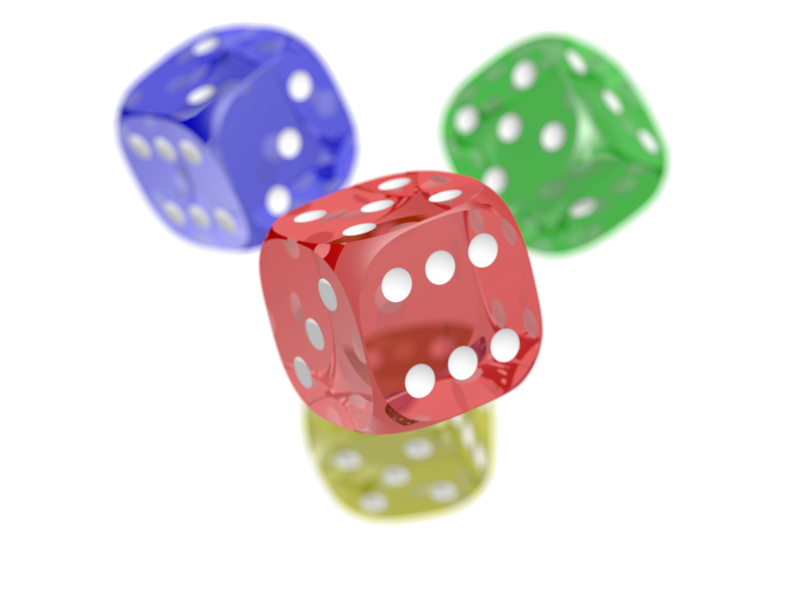
\includegraphics[width=4cm]{img_1.png}
\caption{alt text}
\end{figure}

Here is text

\begin{itemize}
\tightlist
\item
  \(X + Y\)
\item
  \(Z\)
\item
  List3
\end{itemize}

\[x = \frac{1}{2}\]
\end{frame}

\begin{frame}{Ecuaciones junto con texto:}
\protect\hypertarget{ecuaciones-junto-con-texto}{}
Un grafo \(G(p, n)\) \ldots{} \(\text{Ec. normal:} \sum_i^j\)
\[\text{Ec. centrada:} \sum_i^j\]

\begin{equation}
x^2 + x
\end{equation}
\end{frame}

\hypertarget{notaciuxf3n-asintotica}{%
\section{Notación Asintotica}\label{notaciuxf3n-asintotica}}

\begin{frame}{Video con loop}
\protect\hypertarget{video-con-loop}{}
Video 1

\centering
\includemedia[
  width=0.4\linewidth,
  totalheight=0.225\linewidth,
  activate=pageopen,
  passcontext,  %show VPlayer's right-click menu
  addresource=seq2seq_1.mp4,
  flashvars={
    %important: same path as in `addresource'
    source=seq2seq_1.mp4
    &autoPlay=true
    &loop=true
  }
]{\fbox{Click!}}{VPlayer.swf}

\begin{block}{Lista}
\protect\hypertarget{lista}{}
\begin{enumerate}
\tightlist
\item
  A
\item
  B
\item
  C
\end{enumerate}
\end{block}
\end{frame}

\begin{frame}{subsección}
\protect\hypertarget{subsecciuxf3n}{}
\begin{block}{juju}
\protect\hypertarget{juju}{}
\begin{enumerate}
\item ~
  \hypertarget{section}{%
  \subsubsection{}\label{section}}
\end{enumerate}
\end{block}
\end{frame}

\begin{frame}{Lista Incremental}
\protect\hypertarget{lista-incremental}{}
\begin{enumerate}[<+->]
\tightlist
\item
  ¿Hola
\item
  Cómo
\item
  Estan?
\end{enumerate}
\end{frame}

\begin{frame}{Nueva slide}
\protect\hypertarget{nueva-slide}{}
Mi slide nueva
\end{frame}

\hypertarget{nueva-secciuxf3n}{%
\section{Nueva sección}\label{nueva-secciuxf3n}}

\begin{frame}{Slide de la sección 3}
\protect\hypertarget{slide-de-la-secciuxf3n-3}{}
Hola
\end{frame}
